\RequirePackage{luatex85}
\documentclass[tikz]{standalone}
% Default preamble
\usepackage{pgfplots}
\pgfplotsset{compat=newest}
\usepgfplotslibrary{groupplots}
\usepgfplotslibrary{polar}
\usepgfplotslibrary{smithchart}
\usepgfplotslibrary{statistics}
\usepgfplotslibrary{dateplot}
\usepgfplotslibrary{ternary}
\begin{document}
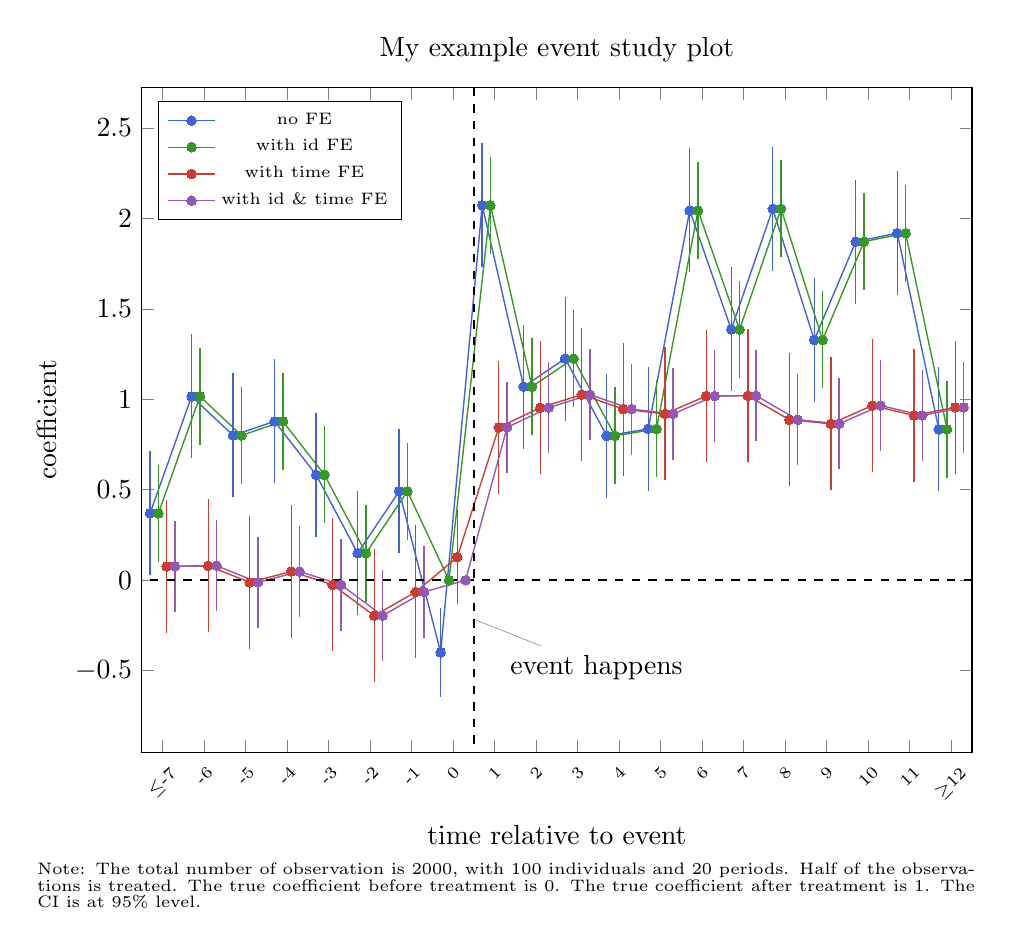
\begin{tikzpicture}
\begin{axis}[title={My example event study plot}, title style={}, xlabel={time relative to event}, xlabel style={}, ylabel={coefficient}, ylabel style={}, xticklabel style={font={\fontsize{6}{6}\selectfont}, rotate={45}}, yticklabel style={}, width={300pt}, height={240pt}, legend style={font={\fontsize{6}{6}\selectfont}, at={(0.02, 0.98)}, anchor={north west}}, symbolic x coords={$\leq$-7,-6,-5,-4,-3,-2,-1,0,1,2,3,4,5,6,7,8,9,10,11,$\geq$12}, xtick={$\leq$-7,-6,-5,-4,-3,-2,-1,0,1,2,3,4,5,6,7,8,9,10,11,$\geq$12}, xmin={{[normalized]-0.5}}, xmax={{[normalized]19.5}}, scale only axis]
    \addplot[mark={*}, mark options={mark size={1.75pt}, line width={0pt}, fill={rgb,255: red, 64; green, 99; blue, 216}, fill opacity={1}, draw={rgb,255: red, 64; green, 99; blue, 216}, draw opacity={1}}, error bars/error mark={none}, error bars/error mark options={mark size={2.0pt}, solid, line width={0.6pt}, fill={rgb,255: red, 64; green, 99; blue, 216}, fill opacity={1}, draw={rgb,255: red, 64; green, 99; blue, 216}, draw opacity={1}}, error bars/error bar style={draw={rgb,255: red, 64; green, 99; blue, 216}, draw opacity={1}, solid, line width={0.5pt}}, draw={rgb,255: red, 64; green, 99; blue, 216}, draw opacity={1}, line width={0.5pt}, error bars/y dir={both}, error bars/y explicit, x filter/.code={{\pgfmathadd{\pgfmathresult}{-0.30000000000000004}}}]
        coordinates {
            ($\leq$-7,0.3697) +- (0,0.34262)
            (-6,1.0162) +- (0,0.34262)
            (-5,0.8004) +- (0,0.34262)
            (-4,0.8779) +- (0,0.34262)
            (-3,0.5828) +- (0,0.34262)
            (-2,0.1494) +- (0,0.34262)
            (-1,0.4916) +- (0,0.34262)
            (0,-0.3985) +- (0,0.24534)
            (1,2.0726) +- (0,0.34262)
            (2,1.0699) +- (0,0.34262)
            (3,1.2251) +- (0,0.34262)
            (4,0.7977) +- (0,0.34262)
            (5,0.8365) +- (0,0.34262)
            (6,2.0437) +- (0,0.34262)
            (7,1.3859) +- (0,0.34262)
            (8,2.0529) +- (0,0.34262)
            (9,1.3283) +- (0,0.34262)
            (10,1.8714) +- (0,0.34262)
            (11,1.918) +- (0,0.34262)
            ($\geq$12,0.8338) +- (0,0.34262)
        }
        ;
    \addlegendentry {no FE}
    \addplot[mark={*}, mark options={mark size={1.75pt}, line width={0pt}, fill={rgb,255: red, 56; green, 152; blue, 38}, fill opacity={1}, draw={rgb,255: red, 56; green, 152; blue, 38}, draw opacity={1}}, error bars/error mark={none}, error bars/error mark options={mark size={2.0pt}, solid, line width={0.6pt}, fill={rgb,255: red, 56; green, 152; blue, 38}, fill opacity={1}, draw={rgb,255: red, 56; green, 152; blue, 38}, draw opacity={1}}, error bars/error bar style={draw={rgb,255: red, 56; green, 152; blue, 38}, draw opacity={1}, solid, line width={0.5pt}}, draw={rgb,255: red, 56; green, 152; blue, 38}, draw opacity={1}, line width={0.5pt}, error bars/y dir={both}, error bars/y explicit, x filter/.code={{\pgfmathadd{\pgfmathresult}{-0.10000000000000003}}}]
        coordinates {
            ($\leq$-7,0.3697) +- (0,0.26849)
            (-6,1.0162) +- (0,0.26849)
            (-5,0.8004) +- (0,0.26849)
            (-4,0.8779) +- (0,0.26849)
            (-3,0.5828) +- (0,0.26849)
            (-2,0.1494) +- (0,0.26849)
            (-1,0.4916) +- (0,0.26849)
            (0,0.0) +- (0,0.0)
            (1,2.0726) +- (0,0.26849)
            (2,1.0699) +- (0,0.26849)
            (3,1.2251) +- (0,0.26849)
            (4,0.7977) +- (0,0.26849)
            (5,0.8365) +- (0,0.26849)
            (6,2.0437) +- (0,0.26849)
            (7,1.3859) +- (0,0.26849)
            (8,2.0529) +- (0,0.26849)
            (9,1.3283) +- (0,0.26849)
            (10,1.8714) +- (0,0.26849)
            (11,1.918) +- (0,0.26849)
            ($\geq$12,0.8338) +- (0,0.26849)
        }
        ;
    \addlegendentry {with id FE}
    \addplot[mark={*}, mark options={mark size={1.75pt}, line width={0pt}, fill={rgb,255: red, 203; green, 60; blue, 51}, fill opacity={1}, draw={rgb,255: red, 203; green, 60; blue, 51}, draw opacity={1}}, error bars/error mark={none}, error bars/error mark options={mark size={2.0pt}, solid, line width={0.6pt}, fill={rgb,255: red, 203; green, 60; blue, 51}, fill opacity={1}, draw={rgb,255: red, 203; green, 60; blue, 51}, draw opacity={1}}, error bars/error bar style={draw={rgb,255: red, 203; green, 60; blue, 51}, draw opacity={1}, solid, line width={0.5pt}}, draw={rgb,255: red, 203; green, 60; blue, 51}, draw opacity={1}, line width={0.5pt}, error bars/y dir={both}, error bars/y explicit, x filter/.code={{\pgfmathadd{\pgfmathresult}{0.09999999999999998}}}]
        coordinates {
            ($\leq$-7,0.0765) +- (0,0.36713)
            (-6,0.08) +- (0,0.36713)
            (-5,-0.0117) +- (0,0.36713)
            (-4,0.0483) +- (0,0.36713)
            (-3,-0.0258) +- (0,0.36713)
            (-2,-0.1958) +- (0,0.36713)
            (-1,-0.0647) +- (0,0.36713)
            (0,0.1269) +- (0,0.25966)
            (1,0.8448) +- (0,0.36713)
            (2,0.9533) +- (0,0.36713)
            (3,1.0256) +- (0,0.36713)
            (4,0.9455) +- (0,0.36713)
            (5,0.9192) +- (0,0.36713)
            (6,1.0183) +- (0,0.36713)
            (7,1.02) +- (0,0.36713)
            (8,0.887) +- (0,0.36713)
            (9,0.8643) +- (0,0.36713)
            (10,0.9657) +- (0,0.36713)
            (11,0.9106) +- (0,0.36713)
            ($\geq$12,0.9555) +- (0,0.36713)
        }
        ;
    \addlegendentry {with time FE}
    \addplot[mark={*}, mark options={mark size={1.75pt}, line width={0pt}, fill={rgb,255: red, 149; green, 88; blue, 178}, fill opacity={1}, draw={rgb,255: red, 149; green, 88; blue, 178}, draw opacity={1}}, error bars/error mark={none}, error bars/error mark options={mark size={2.0pt}, solid, line width={0.6pt}, fill={rgb,255: red, 149; green, 88; blue, 178}, fill opacity={1}, draw={rgb,255: red, 149; green, 88; blue, 178}, draw opacity={1}}, error bars/error bar style={draw={rgb,255: red, 149; green, 88; blue, 178}, draw opacity={1}, solid, line width={0.5pt}}, draw={rgb,255: red, 149; green, 88; blue, 178}, draw opacity={1}, line width={0.5pt}, error bars/y dir={both}, error bars/y explicit, x filter/.code={{\pgfmathadd{\pgfmathresult}{0.3}}}]
        coordinates {
            ($\leq$-7,0.0765) +- (0,0.25222)
            (-6,0.08) +- (0,0.25222)
            (-5,-0.0117) +- (0,0.25222)
            (-4,0.0483) +- (0,0.25222)
            (-3,-0.0258) +- (0,0.25222)
            (-2,-0.1958) +- (0,0.25222)
            (-1,-0.0647) +- (0,0.25222)
            (0,0.0) +- (0,0.0)
            (1,0.8448) +- (0,0.25222)
            (2,0.9533) +- (0,0.25222)
            (3,1.0256) +- (0,0.25222)
            (4,0.9455) +- (0,0.25222)
            (5,0.9192) +- (0,0.25222)
            (6,1.0183) +- (0,0.25222)
            (7,1.02) +- (0,0.25222)
            (8,0.887) +- (0,0.25222)
            (9,0.8643) +- (0,0.25222)
            (10,0.9657) +- (0,0.25222)
            (11,0.9106) +- (0,0.25222)
            ($\geq$12,0.9555) +- (0,0.25222)
        }
        ;
    \addlegendentry {with id \& time FE}
    \draw[dashed, black, line width={0.75}] ({rel axis cs:1,0}|-{axis cs:{[normalized]0},0}) -- ({rel axis cs:0,0}|-{axis cs:{[normalized]0},0});
    \draw[dashed, black, line width={0.75}] ({rel axis cs:0.4,0}|-{rel axis cs:0,1}) -- ({rel axis cs:0.4,0}|-{rel axis cs:0,0});
    \draw node[pin=-45:{event happens}, inner sep=0, outer sep=0] at ({rel axis cs:0.4, 0.2}) {};\end{axis}
\newdimen\notewidth
                    \pgfextractx{\notewidth}{\pgfpointdiff{\pgfpointanchor{current bounding box}{west}}
                    {\pgfpointanchor{current bounding box}{east}}}\draw node[text width={\the\notewidth}, anchor={north west}, at={(current axis.outer south west)}, align={left}, font={\fontsize{6}{6}\selectfont}] {Note: The total number of observation is 2000, with 100 individuals and 20 periods. Half of the observations is treated. The true coefficient before treatment is 0. The true coefficient after treatment is 1. The CI is at 95\% level.};
\end{tikzpicture}
\end{document}
